%% graph G
\subfigure[$G$]{
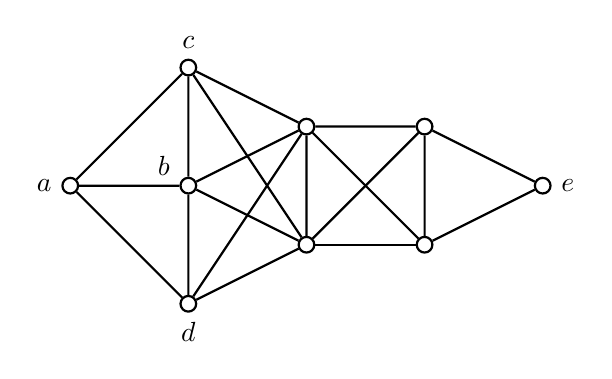
\begin{tikzpicture}
[nodedecorate/.style={shape=circle,inner sep=2pt,draw,thick},%
  linedecorate/.style={-,thick}, scale=1.5]
%% nodes or vertices
\foreach \nodename/\x/\y in {a/0/1, b/1/1, c/1/2, d/1/0, 1/2/1.5,
  2/2/0.5, 3/3/1.5, 4/3/0.5, e/4/1}
{
  \node (\nodename) at (\x,\y) [nodedecorate] {};
}
\foreach \nodename/\direction/\navigate in {a/left/west,
  b/above left/west, c/above/north, d/below/south, e/right/east}
{
  \node [\direction] at (\nodename.\navigate) {$\nodename$};
}
%% edges or lines
\path
\foreach \startnode/\endnode in {a/b, a/c, a/d, b/c, b/d, b/1, b/2,
  c/1, c/2, d/1, d/2, 1/2, 1/3, 1/4, 2/3, 2/4, 3/4, 3/e, 4/e}
{
  (\startnode) edge[linedecorate] node {} (\endnode)
};
\end{tikzpicture}
}
%%
%% vertex deletion subgraph G - {b}
\subfigure[$G - \{b\}$]{
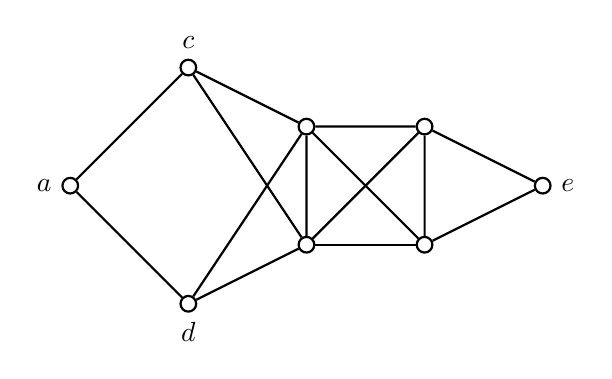
\begin{tikzpicture}
[nodedecorate/.style={shape=circle,inner sep=2pt,draw,thick},%
  linedecorate/.style={-,thick}, scale=1.5]
%% nodes or vertices
\foreach \nodename/\x/\y in {a/0/1, c/1/2, d/1/0, 1/2/1.5, 2/2/0.5,
  3/3/1.5, 4/3/0.5, e/4/1}
{
  \node (\nodename) at (\x,\y) [nodedecorate] {};
}
\foreach \nodename/\direction/\navigate in {a/left/west,
  c/above/north, d/below/south, e/right/east}
{
  \node [\direction] at (\nodename.\navigate) {$\nodename$};
}
%% edges or lines
\path
\foreach \startnode/\endnode in {a/c, a/d, c/1, c/2, d/1, d/2, 1/2,
  1/3, 1/4, 2/3, 2/4, 3/4, 3/e, 4/e}
{
  (\startnode) edge[linedecorate] node {} (\endnode)
};
\end{tikzpicture}
}
%%
%% vertex deletion subgraph G - {a,b}
\subfigure[$G - \{a, b\}$]{
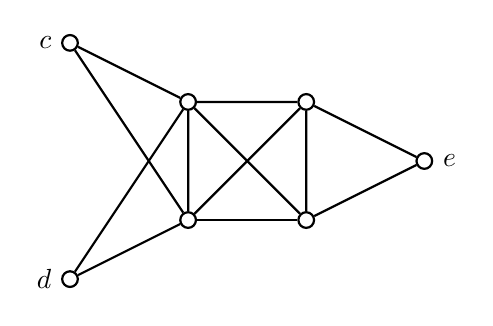
\begin{tikzpicture}
[nodedecorate/.style={shape=circle,inner sep=2pt,draw,thick},%
  linedecorate/.style={-,thick}, scale=1.5]
%% nodes or vertices
\foreach \nodename/\x/\y in {c/1/2, d/1/0, 1/2/1.5, 2/2/0.5, 3/3/1.5,
  4/3/0.5, e/4/1}
{
  \node (\nodename) at (\x,\y) [nodedecorate] {};
}
\foreach \nodename/\direction/\navigate in {c/left/west,
  d/left/west, e/right/east}
{
  \node [\direction] at (\nodename.\navigate) {$\nodename$};
}
%% edges or lines
\path
\foreach \startnode/\endnode in {c/1, c/2, d/1, d/2, 1/2, 1/3, 1/4,
  2/3, 2/4, 3/4, 3/e, 4/e}
{
  (\startnode) edge[linedecorate] node {} (\endnode)
};
\end{tikzpicture}
}
%%
%% vertex deletion subgraph G - {a,b,e}
\subfigure[$G - \{a, b, e\}$]{
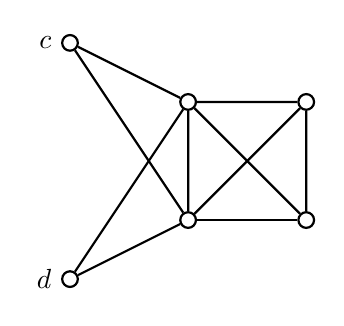
\begin{tikzpicture}
[nodedecorate/.style={shape=circle,inner sep=2pt,draw,thick},%
  linedecorate/.style={-,thick}, scale=1.5]
%% nodes or vertices
\foreach \nodename/\x/\y in {c/1/2, d/1/0, 1/2/1.5, 2/2/0.5, 3/3/1.5,
  4/3/0.5}
{
  \node (\nodename) at (\x,\y) [nodedecorate] {};
}
\foreach \nodename/\direction/\navigate in {c/left/west,
  d/left/west}
{
  \node [\direction] at (\nodename.\navigate) {$\nodename$};
}
%% edges or lines
\path
\foreach \startnode/\endnode in {c/1, c/2, d/1, d/2, 1/2, 1/3, 1/4,
  2/3, 2/4, 3/4}
{
  (\startnode) edge[linedecorate] node {} (\endnode)
};
\end{tikzpicture}
}
%%
%% vertex deletion subgraph G - {a,b,c,d,e}
\subfigure[$G - \{a, b, c, d, e\}$]{

\begin{tikzpicture}
[nodedecorate/.style={shape=circle,inner sep=2pt,draw,thick},%
  linedecorate/.style={-,thick}, scale=1.5]
%% nodes or vertices
\foreach \nodename/\x/\y in {1/2/1.5, 2/2/0.5, 3/3/1.5, 4/3/0.5} {
  \node (\nodename) at (\x,\y) [nodedecorate] {};
}
%% a stub node that should not be visible
\node (stubLeft) at (0,1.5) [] {};
\node (stubRight) at (5,1.5) [] {};
%% edges or lines
\path
\foreach \startnode/\endnode in {1/2, 1/3, 1/4, 2/3, 2/4, 3/4} {
  (\startnode) edge[linedecorate] node {} (\endnode)
};
\end{tikzpicture}
}
